\documentclass{article}
\usepackage[utf8]{inputenc}
\usepackage{graphicx}
\graphicspath{ {./images/} }
\title{CS3093D Networks Laboratory  - Assignment 1}
\author{Anandu B Ajith - B180288CS}
\date{16 January 2022}

\begin{document}

% 
% export PS1="anandu_b180288cs $ "
% 

\maketitle

\section{ping}
`ping` command can be used to check connectivity between client and host. `ping` sends an ICMP ( Internet Control Message protocol) Echo Request and waits for response. In case of a successful connection ICMP Echo Reply is received for every request. The output also contains the amount of time the ICMP packet takes to reach destination and return.

\begin{figure}[ht]
    \centering
    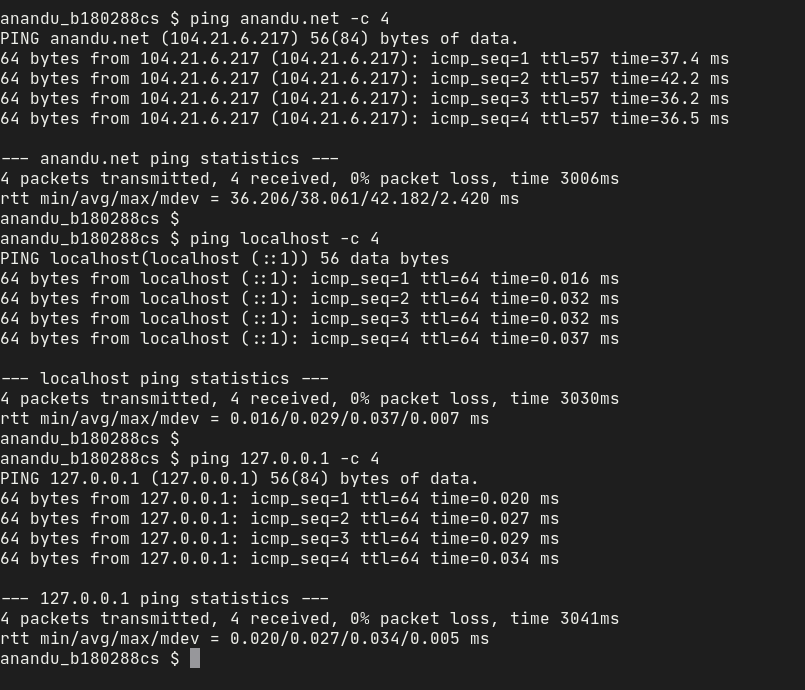
\includegraphics[width=1.0\textwidth]{images/ping.png}
\end{figure}
\pagebreak
\section{tracert/traceroute}

`traceroute` command can be used to trace the route which a packet takes to reach it's destination. It displays all the hops which packet visits, and the latency between each hop. This tool can be used to debug network issues where the packet is failing to reach destination
\begin{figure}[ht]
    \centering
    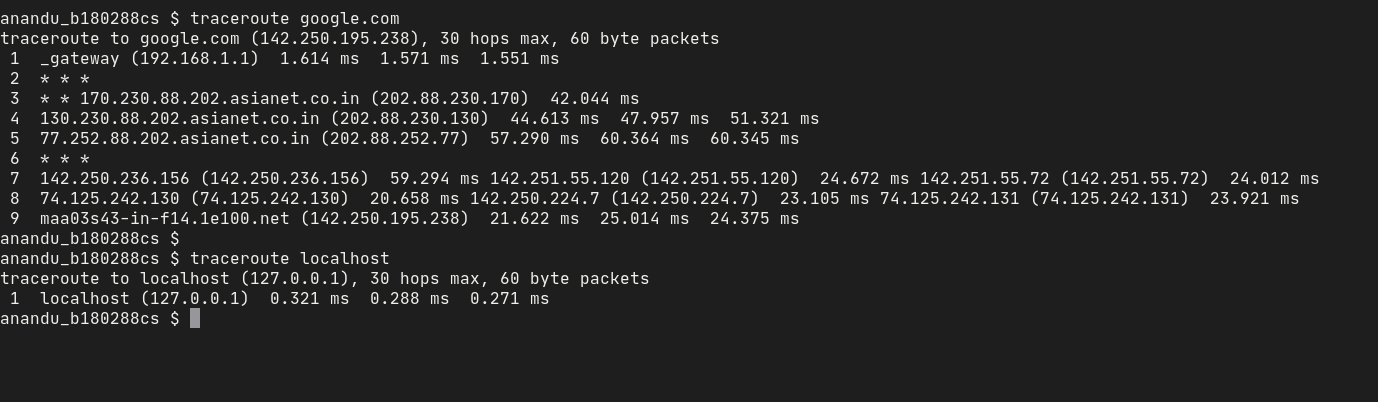
\includegraphics[width=1.0\textwidth]{images/traceroute.png}
\end{figure}


\pagebreak
\section{ip/ifconifg/ipconfig}
`ip` command is often used to troubleshoot network connectivity issues, and to find out the IP address of the system. It is also used to bring network interfaces up and down.`ip a` can be used to display the available interfaces and their configuration. `ip r` can be used to display and manipulate the routing table.

\begin{figure}[ht]
    \centering
    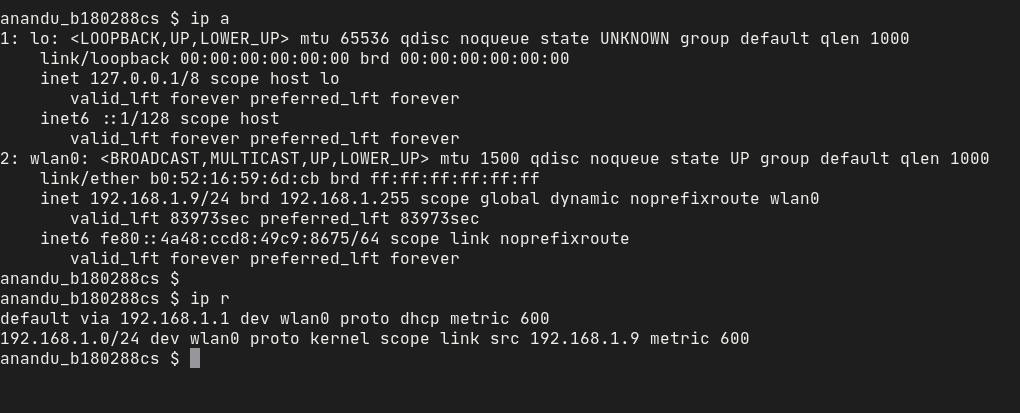
\includegraphics[width=1.0\textwidth]{images/ip.png}
\end{figure}
\pagebreak

\section{dig/nslookup/host}
DNS maps domain names to it's corresponding IP address. `dig` can be used to troubleshoot DNS lookups.
`dig +trace anandu.net` can be used to make dig output verbose with all the queries it performs.
\begin{figure}[ht]
    \centering
    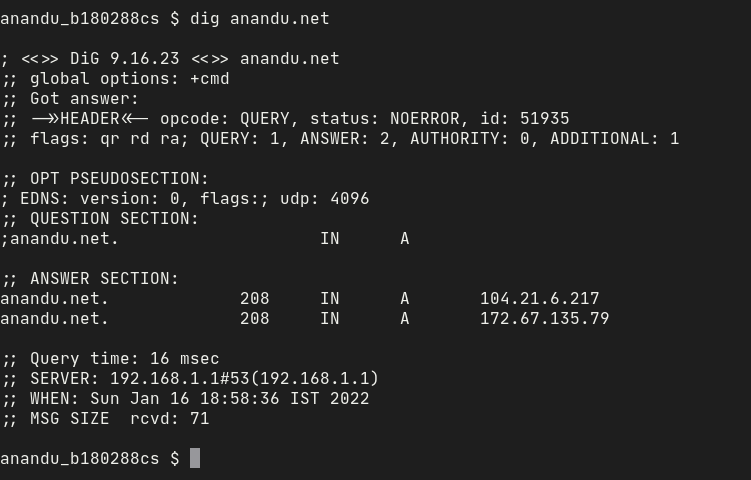
\includegraphics[width=1.0\textwidth]{images/dig.png}
\end{figure}
\pagebreak

\section{whois}
`whois` database contains the listings about the ownership of domains. ICANN regulates the domain name registration and ownership, but the list of records is held by many compaines, known as registries such that anyone can query the list of records. `whois` record contains the contact information of the domain owner.
\begin{figure}[ht]
    \centering
    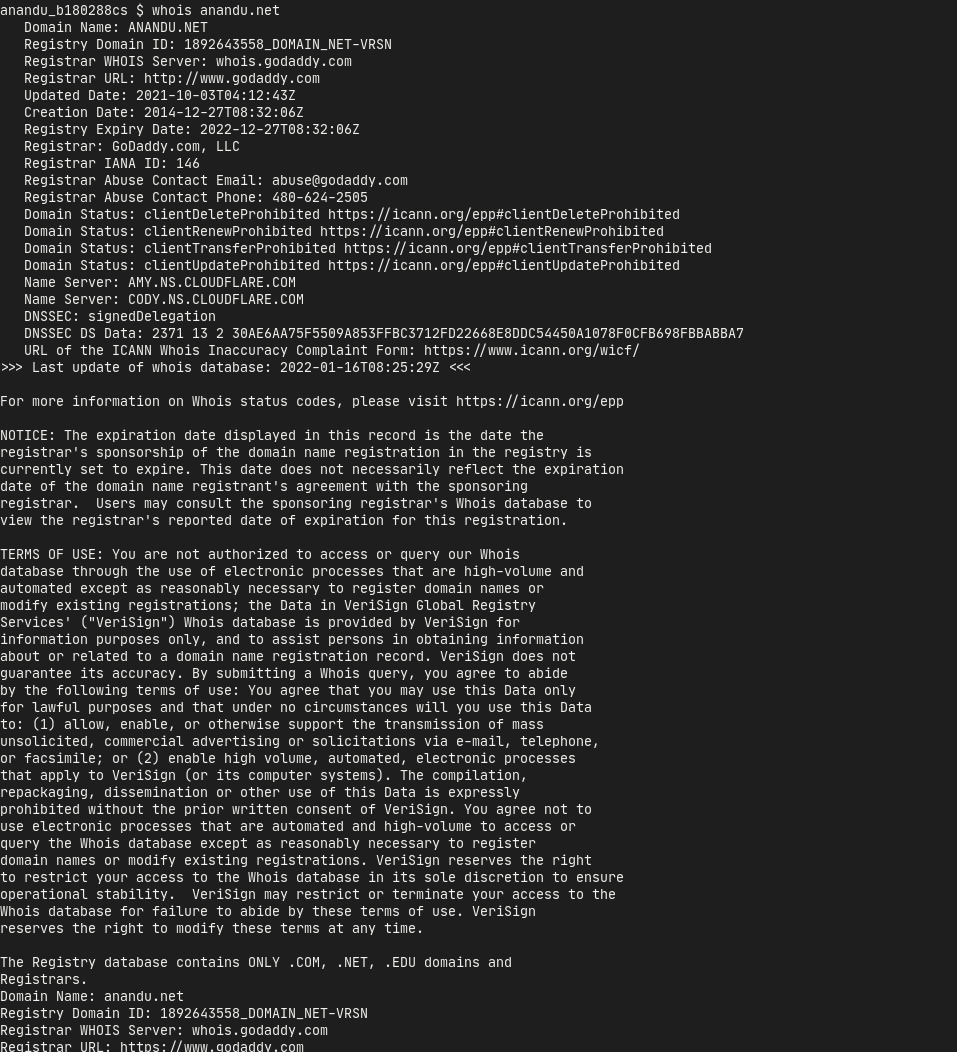
\includegraphics[width=1.0\textwidth]{images/whois.png}
\end{figure}
\pagebreak

\section{route}
Routing table contains information on how the packet should be transferred. It is used by routers and gateways to track paths. Once the packet reaches the next hop, routing table is again consulted to route the packet forward. `route` command is used to manipulate the routing table.
\begin{figure}[ht]
    \centering
    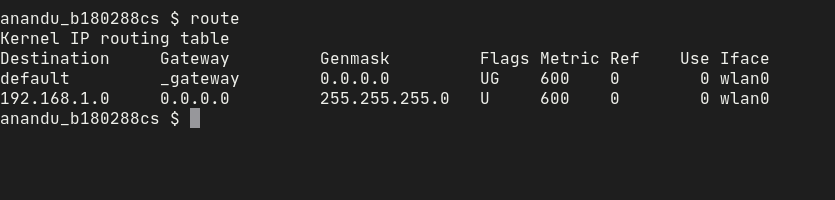
\includegraphics[width=1.0\textwidth]{images/route.png}
\end{figure}
\pagebreak

\section{tcpdump}
`tcpdump` can be used to capture and analyze network traffic going through the system. It is normally used to troubleshoot and monitor the network for security issues. `tcpdump` can output theh data as .pcap file which can be opened in tools like WireShark.
\begin{figure}[ht]
    \centering
    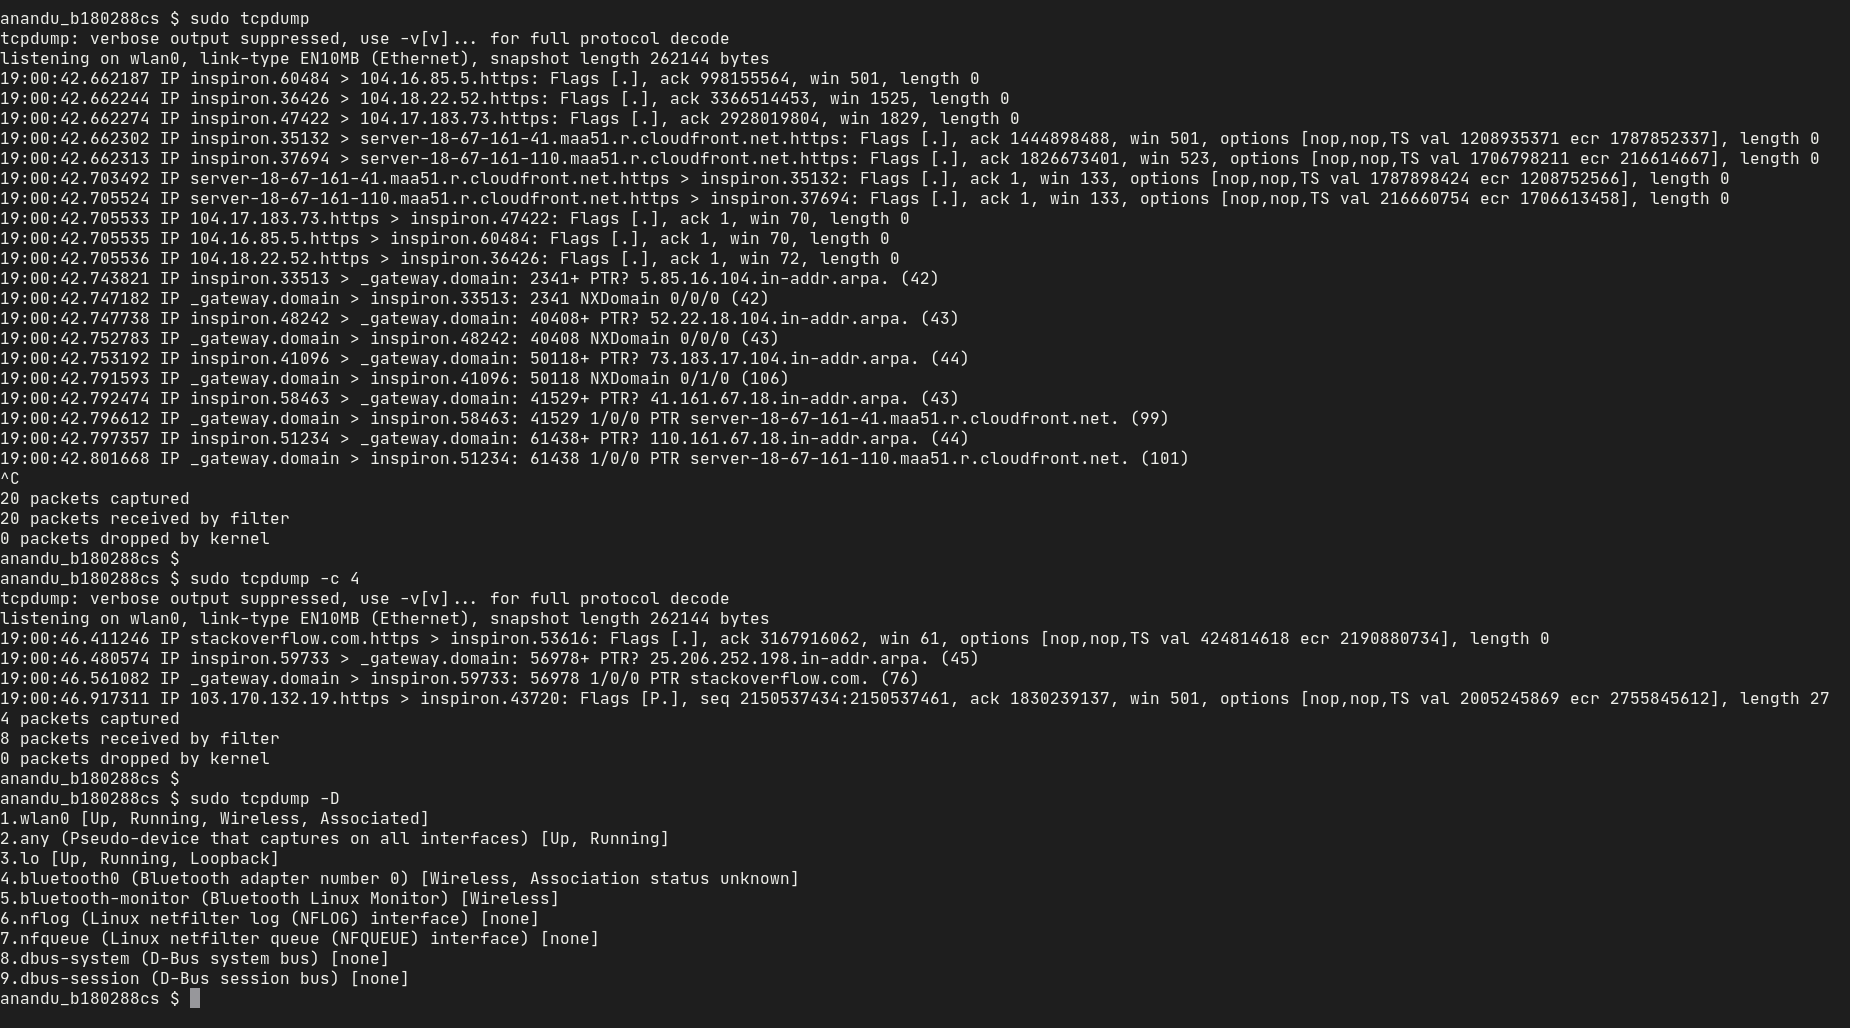
\includegraphics[width=1.0\textwidth]{images/tcpdump.png}
\end{figure}
\pagebreak

\section{netstat/ss}
`ss` ( socket stats ) can be used to get detailed information about how Linux is communicating through sockets. `ss -tnlp` can be used to display the active listeners, and the program which is listening. `ss -s` displays the overall connection summary.
\begin{figure}[ht]
    \centering
    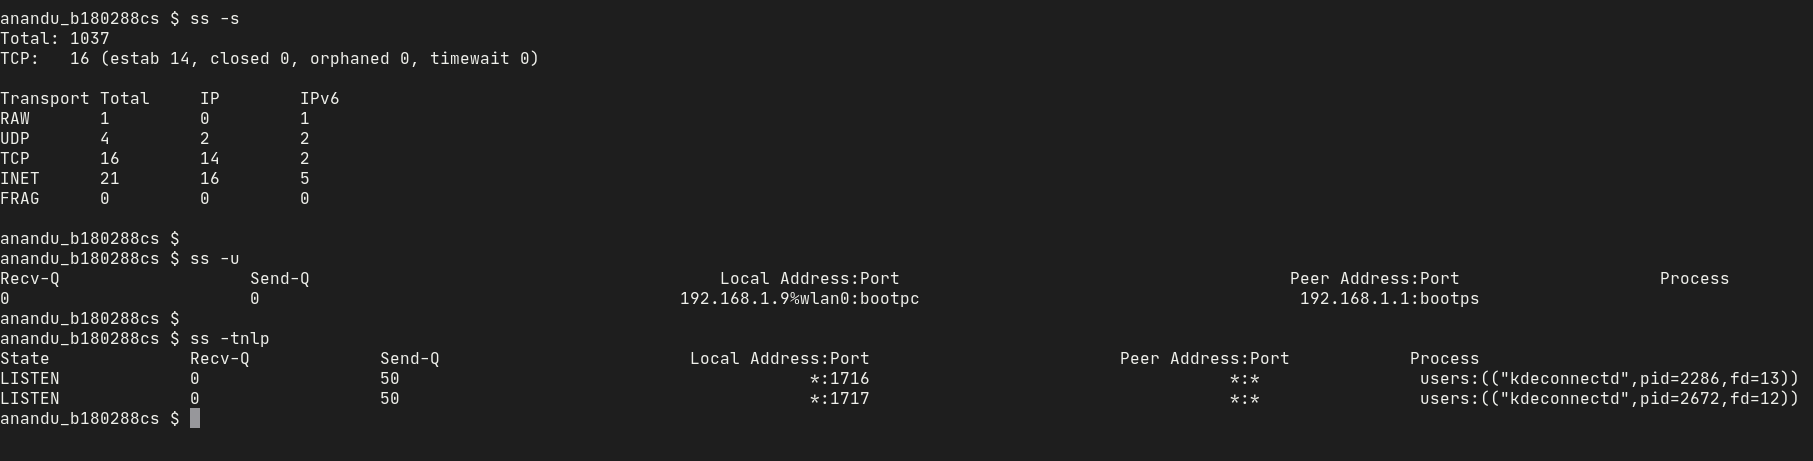
\includegraphics[width=1.0\textwidth]{images/ss.png}
\end{figure}
\pagebreak

\section{dstat}
`dstat` is used to retrive statistics from system components like CPU, Memory, network connections, IO devices etc. Used by sysadmins to retrive information about the system to if there is anything misbehaving.  
\begin{figure}[ht]
    \centering
    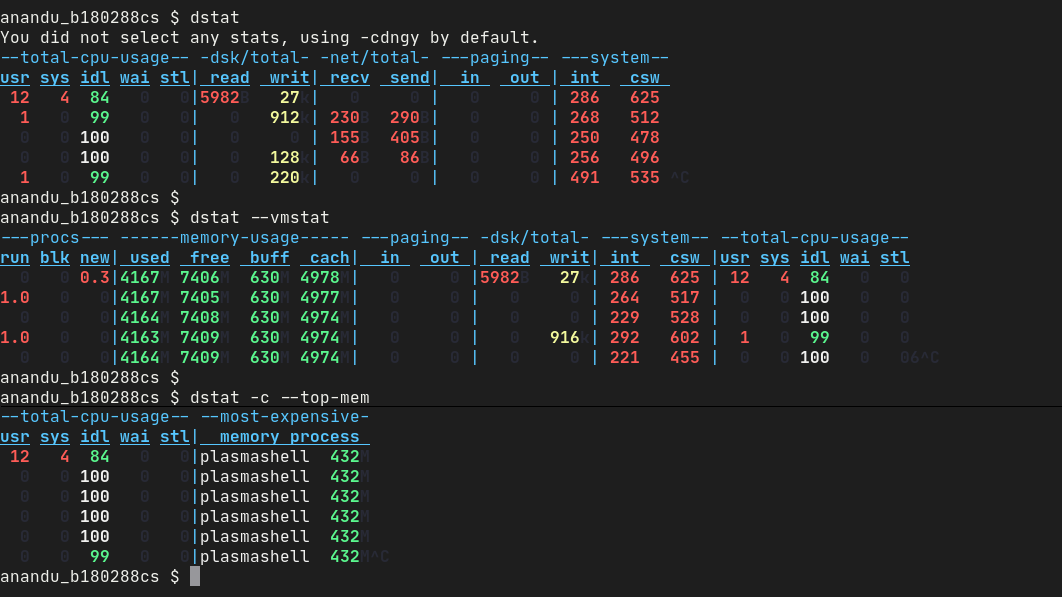
\includegraphics[width=1.0\textwidth]{images/dstat.png}
\end{figure}
\pagebreak

\section{ifstat}
Similar to `dstat`, `ifstat` can be used to display network interface statistics. The tool outputs the difference between the current and previous calls.
\begin{figure}[ht]
    \centering
    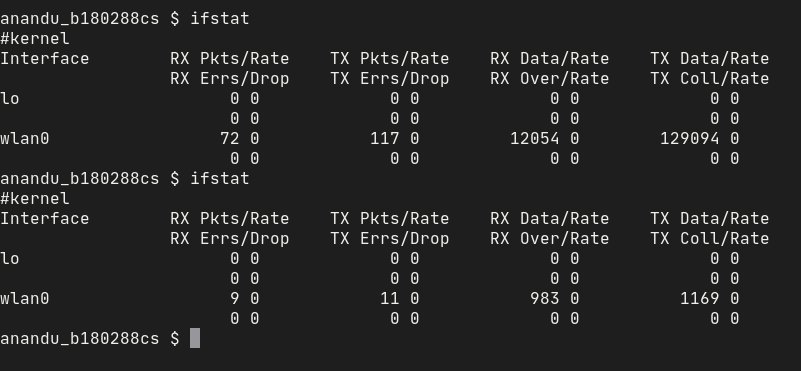
\includegraphics[width=1.0\textwidth]{images/ifstat.png}
\end{figure}
\pagebreak

\section{wget}
`wget` is a command line program used to download files from various protocols like HTTP, HTTPS and FTP. It supports downloading multiple files, resuming broken transfers, limiting the download bandwidth, and website mirroring.6
\begin{figure}[ht]
    \centering
    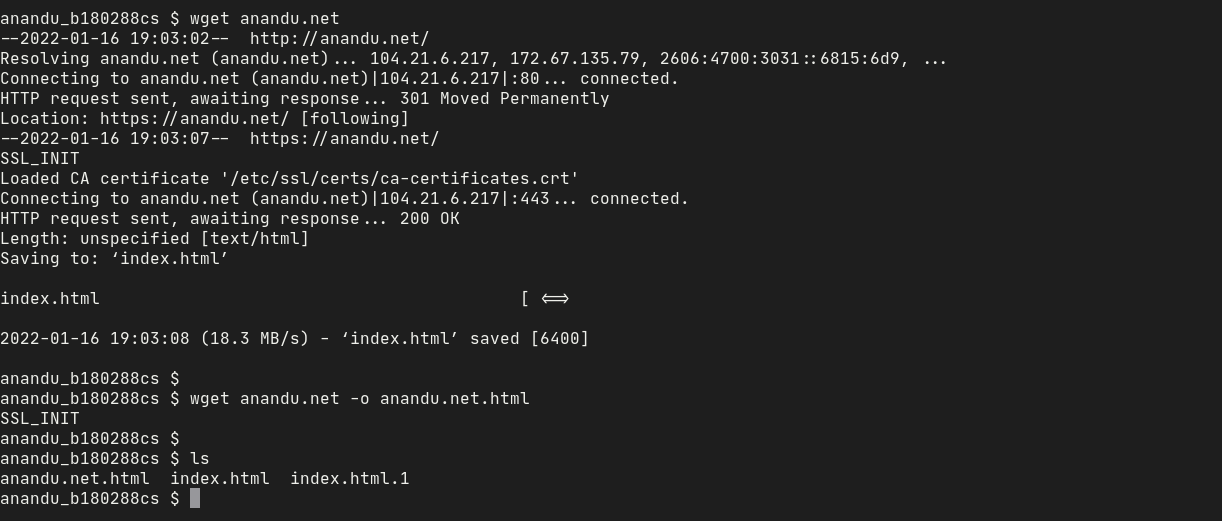
\includegraphics[width=1.0\textwidth]{images/wget.png}
\end{figure}
\pagebreak

\section{tracepath}
`tracepath` is a replacement for `traceroute` command which does not require superuser privileges. It can be used to trace the path which a packet takes to reach it's destination in the network.
\begin{figure}[ht]
    \centering
    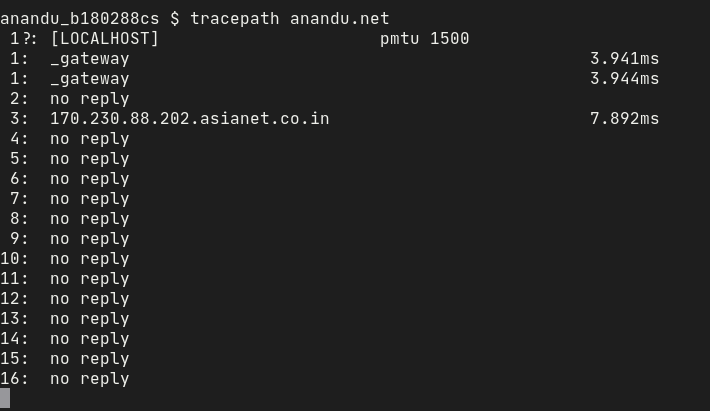
\includegraphics[width=1.0\textwidth]{images/tracepath.png}
\end{figure}
\pagebreak
\end{document}
